\section{Operationsverstärker}
\todo{28.9 Woche 2}
\todo{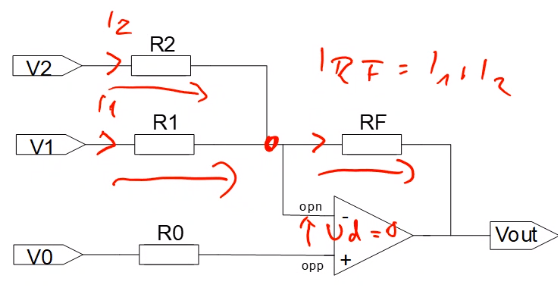
\includegraphics[width=\linewidth]{Images/opamp_todo}}


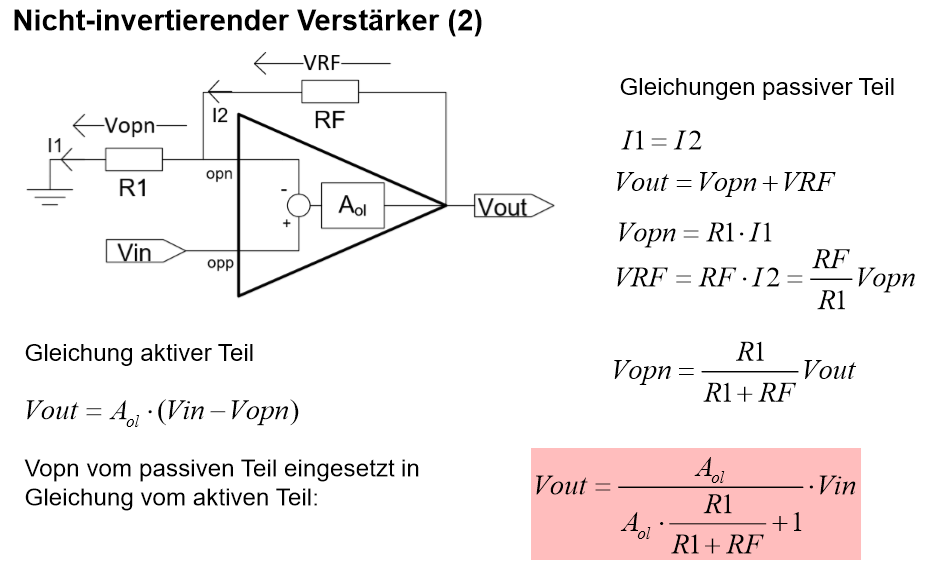
\includegraphics[width=\linewidth]{Images/opamp_negatives_feedback}
Wenn $\frac{1}{A_{ol}} << \frac{R_1}{R_1 + R_F}$, dann gilt auch:
\[
V_{out} = \frac{R_1 + R_F}{R_1} \cdot V_{in}
\]

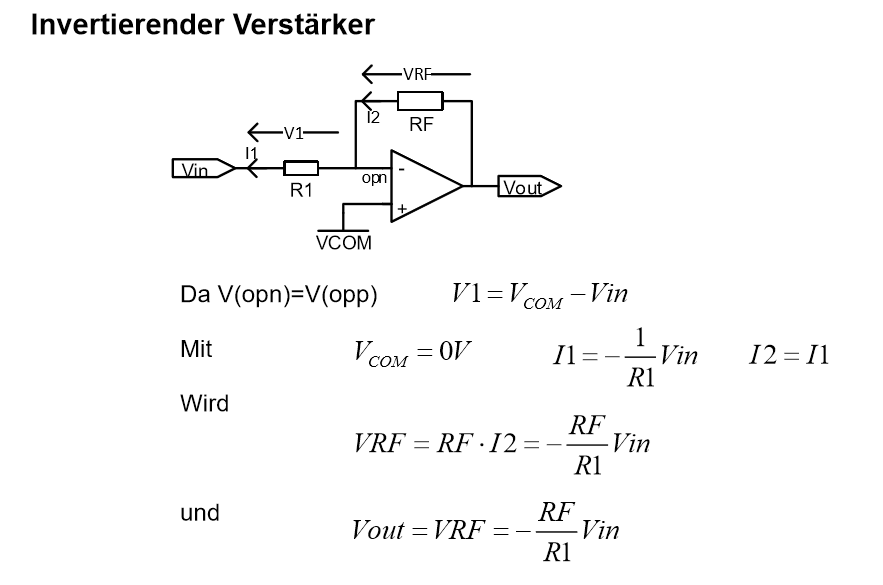
\includegraphics[width=\linewidth]{Images/opamp_invertierendpng}

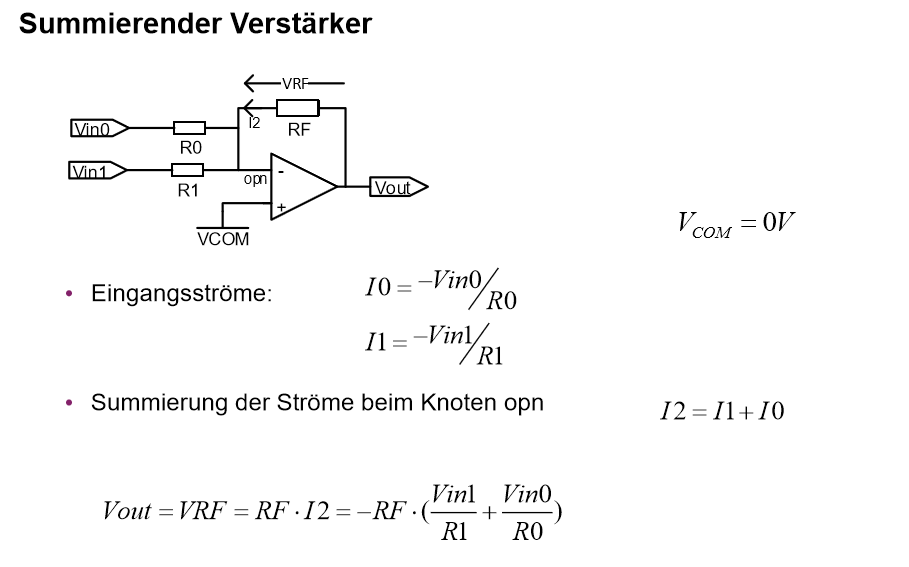
\includegraphics[width=\linewidth]{Images/opamp_summierend}

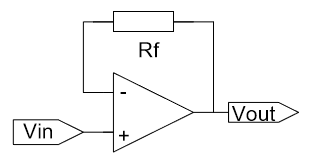
\includegraphics[width=\linewidth]{Images/opamp_buffer}

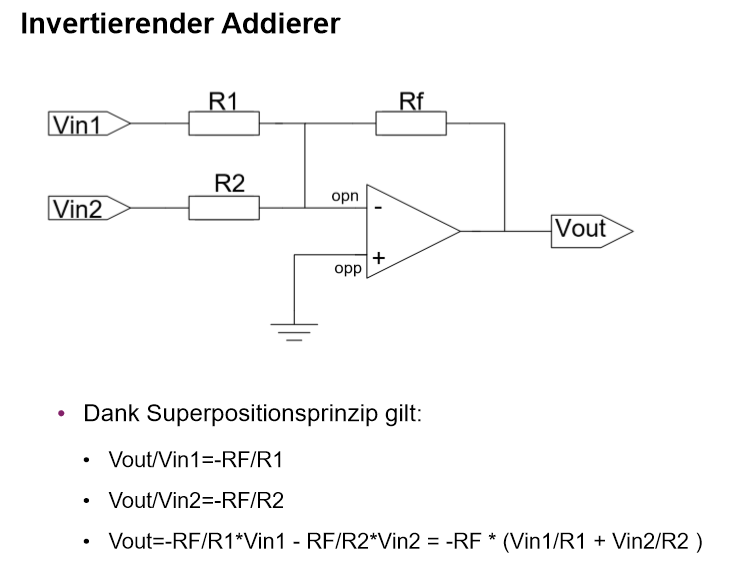
\includegraphics[width=\linewidth]{Images/opamp_invertierend_addierer}

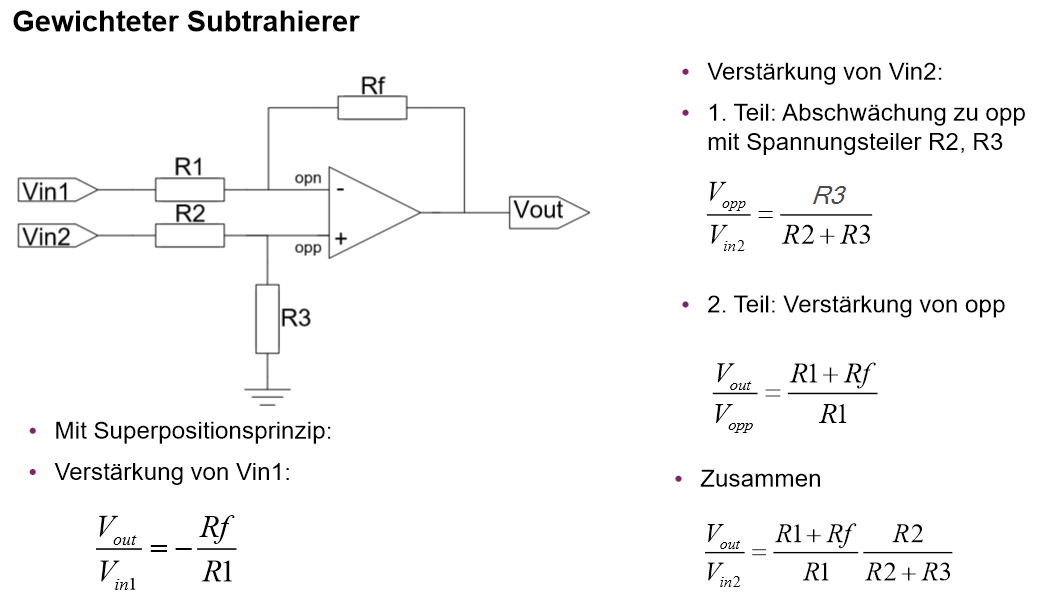
\includegraphics[width=\linewidth]{Images/opamp_invertierend_subtrahierer}

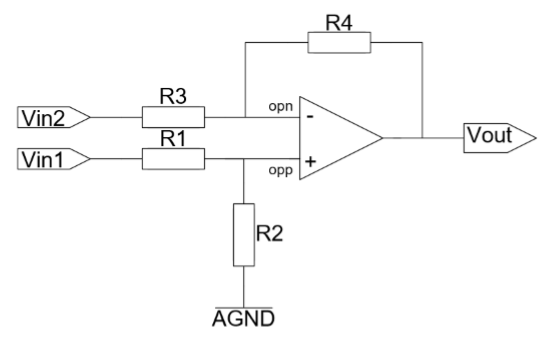
\includegraphics[width=\linewidth]{Images/opamp_differenz}
 
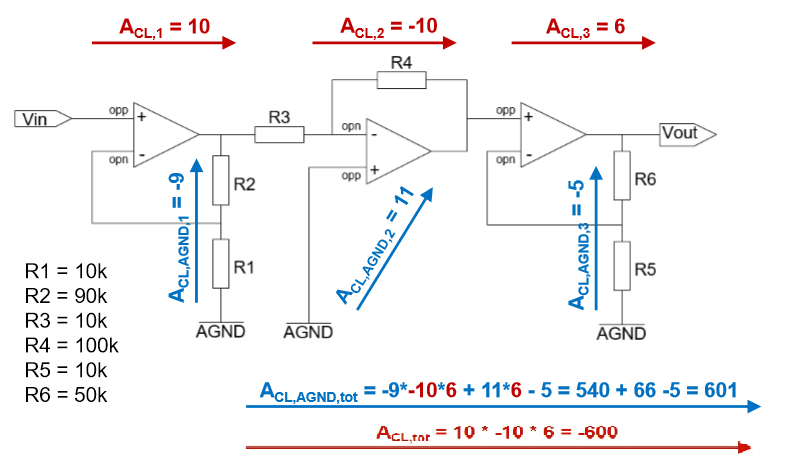
\includegraphics[width=\linewidth]{Images/opamp_mehrstufig}

\todo{5.10 Woche 3}
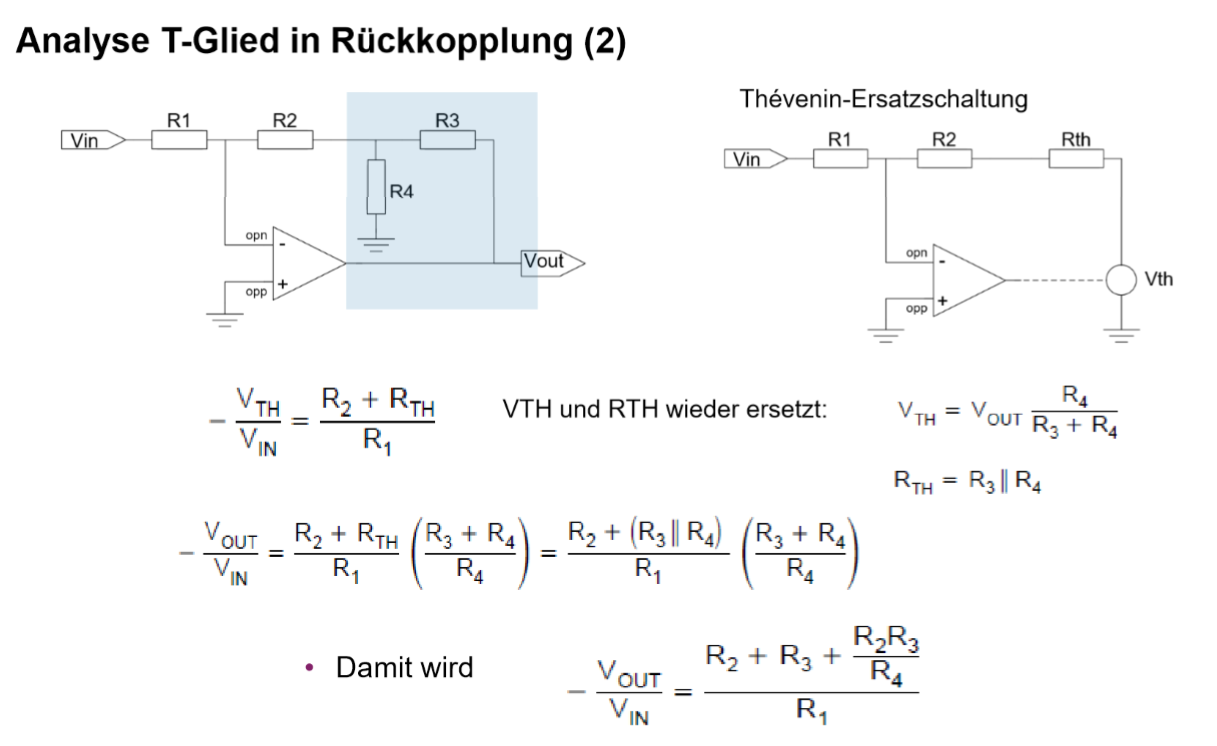
\includegraphics[width=\linewidth]{Images/opamp_t-glied}

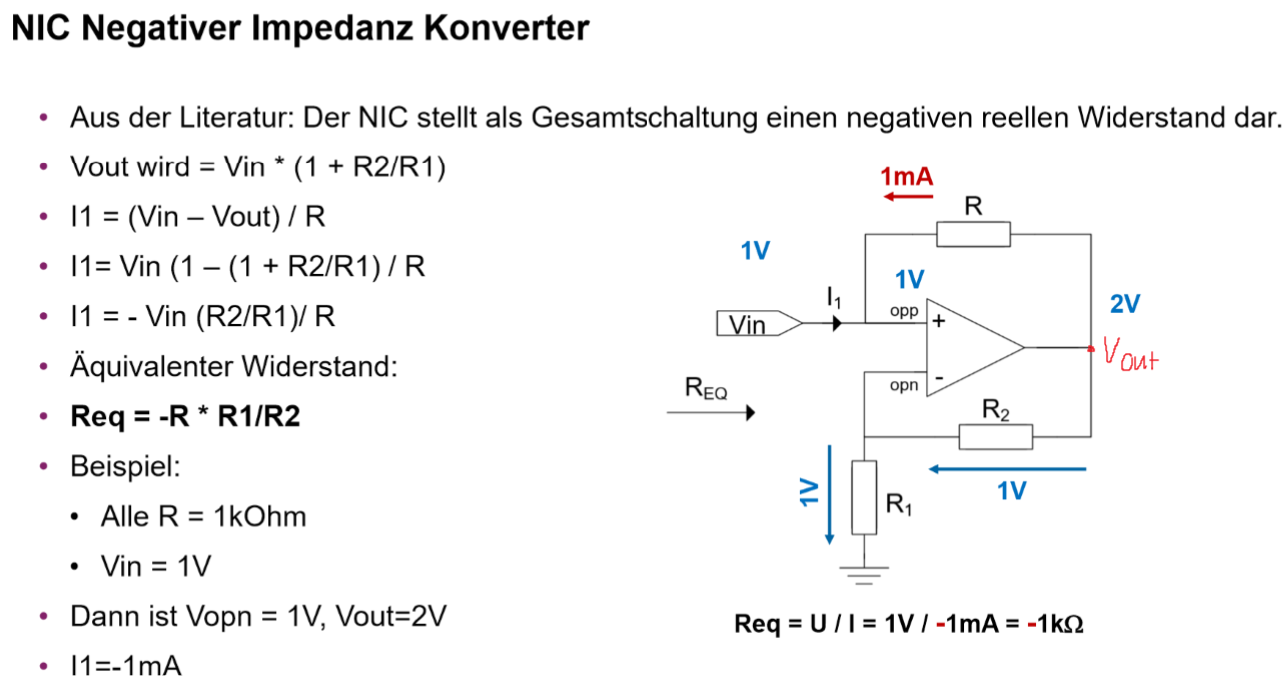
\includegraphics[width=\linewidth]{Images/opamp_nic}


\subsection{Nicht idealer OP}
\todo{5.10 Woche 3}
\begin{enumerate}[nosep]
	\item Offsetspannung\\
	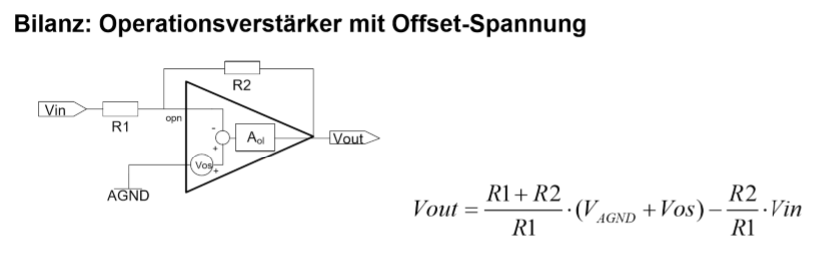
\includegraphics[width=\linewidth]{Images/opamp_offset_spannung}
	
	\item Offset Strom\\
	Eingangswiderstände verkleinern
	\item Arbeitsbereich
	\item Endliche Verstärkung	
\end{enumerate}

\subsection{Dynamische Eigenschaften}
\todo{5.10 Woche 3}
GBP = Gain Bandwidth Product\\
\includegraphics[width=\linewidth]{Images/opamp_dynamische_verstärkung}

Produkt von 3dB-Knickfrequenz (=Bandbreite) und Verstärkung (von pos. Eingang = $\frac{1}{\beta}$) ist konstant

\subsection{Slew-Rate}
\todo{12.10 Woche 4}
Slew-Rate (SW) bezeichnet mögliche Änderungsgeschwindigkeit der Ausgangsspannung
\[
SR = \left|\frac{dV_{out}}{dt}\right|_{max}
\]
